\documentclass[10pt,twocolumn,letterpaper]{article}

\usepackage{cvpr}
\usepackage{times}
\usepackage{epsfig}
\usepackage{graphicx}
\usepackage{amsmath}
\usepackage{amssymb}
\usepackage{subfig}

% Include other packages here, before hyperref.

% If you comment hyperref and then uncomment it, you should delete
% egpaper.aux before re-running latex.  (Or just hit 'q' on the first latex
% run, let it finish, and you should be clear).
%\usepackage[pagebackref=true,breaklinks=true,letterpaper=true,colorlinks,bookmarks=false]{hyperref}

\cvprfinalcopy % *** Uncomment this line for the final submission

\def\cvprPaperID{****} % *** Enter the CVPR Paper ID here
\def\httilde{\mbox{\tt\raisebox{-.5ex}{\symbol{126}}}}

% Pages are numbered in submission mode, and unnumbered in camera-ready
\ifcvprfinal\pagestyle{empty}\fi
\begin{document}

%%%%%%%%% TITLE
\title{Challenges of Object Localization in the ImageNet Dataset}

\author{Siddharth Batra\\
Stanford University\\
Stanford, CA\\
{\tt\small sidbatra@cs.stanford.edu}
% For a paper whose authors are all at the same institution,
% omit the following lines up until the closing ``}''.
% Additional authors and addresses can be added with ``\and'',
% just like the second author.
% To save space, use either the email address or home page, not both
}

\maketitle
\thispagestyle{empty}

%%%%%%%%% ABSTRACT
\begin{abstract}
    
   With ever increasing computational resources and a virtually unlimited online collection of multimedia
   content computer vision research is thriving with innovation like never before. Hence, it seems counterintuitive
   to use constrainted datasets that don't actually capture the true nature of the problem. However, due to its sheer size
   and variety the ImageNet dataset is perhaps the closest representation of the real problem in terms of the variabilty of
   the object attributes such as pose, apperance, lighting, size, viewpoint, shape etc. This paper aims to highlight 
   some of the challenges involved in object localization on a dataset with such high variance in object attributes.
   We present how conventional localization techniques will fail on such datasets, share some experimental insight
   about the dataset and also present a simulation technique for localization approaches to efficiently test different classifiers.
   Finally, we present a boosting inspired localization technique which although isn't state of the art but it shares
   an insight into the kind of methods that should work well on this dataset.

\end{abstract}

%%%%%%%%% BODY TEXT
\section{Introduction}

Over the years, computer vision research has come a long way in identifying
and understanding the challenges associated with truly "solving"
the different facets of the vision problem. This combined with the exponential
growth of computational resources and the vast collections of online multimedia 
has led to a flurry of innovative research works in the last decade.

Amongst this prolific growth of computer vision there has been
critisicm for hand-tailored datasets and performance metrics that do not accurately 
reflect the complexity of the problem at hand.

Although, well labeled datasets such as Caltech101/256 \cite{dataset2,dataset3} and PASCAL
\cite{dataset1} have alleviated the problem to some extent, the sheer number of images
per category in the ImageNet \cite{dataset4} dataset result in an extremely high
variance over object attributes such as color, viewpoint, orientation, size, appearance, pose,
shape etc. Thus, ImageNet and the way its generated make it the closest approximation
to the true variance in real world object attributes. Figure \ref{fig:dataset} gives an
example of variance in the three ImageNet object categories chosen for expertiments
in our work.

The task of object localization involves drawing a tight bounding box around all instances
of an object class within an image. This paper aims to highlight some of the challenges involved in performing object 
localization on the three object categories shown in Figure \ref{fig:dataset}. We start with presenting a reasoning against the use
of conventional object localization techniques on this dataset and follows it with a set of basic
experiments that cement its complexity. A commonly used technique is presented to bypass conventional localization
techniques for testing different classifiers on the data without the explicit need of localization i.e. a 
theoretical simulation of the sliding window approach. Two different feature sets and classifiers are presented and tested
via the simulated sliding window approach. Lastly, a boosting inspired localization strategy is proposed that 
is not perfect but doesn't suffer from the drawbacks discussed of conventional localization techniques.

Although we do not achieve state of the art performance, hopefully these results will give some insight about the kind of 
methods that are most suited for object localization on such a complex dataset.


\begin{figure}[t]
\begin{center}
   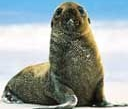
\includegraphics[width=1.0in,height=1.0in]{sea_lion_1.jpg}
   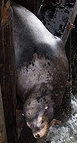
\includegraphics[width=1.0in,height=1.0in]{sea_lion_2.jpg}
   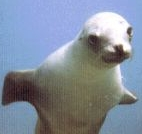
\includegraphics[width=1.0in,height=1.0in]{sea_lion_3.jpg}
\end{center}
\begin{center}
   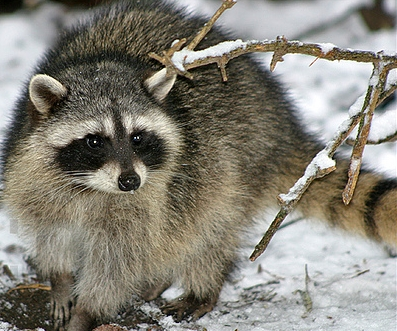
\includegraphics[width=1.0in,height=1.0in]{racoon_1.jpg}
   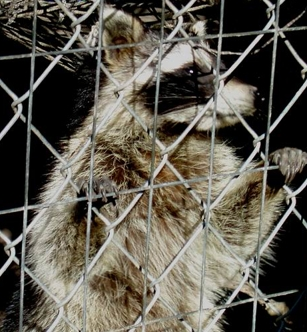
\includegraphics[width=1.0in,height=1.0in]{racoon_2.jpg}
   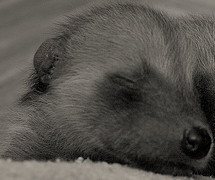
\includegraphics[width=1.0in,height=1.0in]{racoon_3.jpg}
\end{center}
\begin{center}
   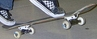
\includegraphics[width=1.0in,height=1.0in]{skate_1.jpg}
   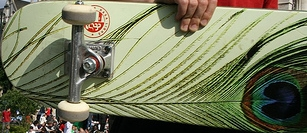
\includegraphics[width=1.0in,height=1.0in]{skate_2.jpg}
   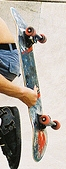
\includegraphics[width=1.0in,height=1.0in]{skate_3.jpg}
\end{center}
   \caption{Example of the high variance in object attributes in the ImageNet dataset. The first row are
   sea lions, followed by racoons and skateboards.}
\label{fig:dataset}
\end{figure}
%-------------------------------------------------------------------------

\section{Previous work}

There has been extensive work done in the areas of single object
recognition and localization using both single and multiple views.
Previous works such as \cite{single1,single2} have used object specific and highly
disciminative features such as SIFT \cite{feature1} to locate rigid objects
from varying viewpoints. Although comendable, these methods rely
on the rigid  geometry and highly discriminative features of the objects
they seek to localize. Hence, such techniques will not be able to accomodate the high
intra class variability and the non-rigid nature of objects such as animals where
the space of all poses can't be quantized into a small enough number to 
apply multiple instances of rigid object classifiers.

A larger body of work in the last few years investigates object categorization for all instances of 
objects of a class under limited variance of object attributes such as shape, 
appearance, size and view point \cite{view1,view2,view3}.

More recently, several novel attempts \cite{multiview1,multiview2,multiview3} have been made to investigate object recognition
from multiple poses with reasonably high apperance variability via a part based approach.

Most of the above works though share great insight about the problem at hand they however use datasets 
that enforce constraints over one or more attributes of an object such as the 
viewpoint, pose or appearance and hence are not a true reflection
of the variance of object attributes in real life.

Since the ImageNet dataset is quite new it is hard to find a good paper that uses it as a dataset and presents some
compeling results. The creators of ImageNet have published \cite{dataset1} a set of results using very basic nearest
neighbour metrics along with a deep analysis of the dataset to highlight its richness and the complexity of the problem at hand.

In this paper we try and present reasons for the failure of conventional localization techniques on the
ImageNet dataset and motivate an alternative strategy that is far from perfect but doesn't suffer from the
drawbacks of existing techniques.


%-------------------------------------------------------------------------

\section{Approach}


\subsection{Conventional localization techniques}

One of the upcoming ways of localizing instances of an object class within an image
is to use a part based model \cite{multiview1}. In this model, we compute the probability of an
object part being found at each interest point in the image. This raw information
is usually churned through a graphical model to get the best possible joint estimate
of the location of an object within an image.This approach works reasonably well
when we make the assumption that an object is rigid and has a set of well defined
parts a subset of which will always be visible. However, if we consider the case of 
non-rigid objects such as animals it will be very hard to learn an accurate model
of each object part since the very term carries a lose definition especially in a
high variance dataset like ImageNet where they will not a consistent appearance 
model of each object part.
The other standard and more commonly used method for object localization is the 
sliding window approach. This involves taking a fixed size window and convolving
it over every location and scale in the given image and evaluating a bag of words
style binary classifier at each location. Although computationally expensive
it has shown great promise especially with rigid objects \cite{multiview4}
One of the fundamental assumptions of the sliding window approach is a very small
variance on the distribution of aspect ratios of the object class thereby ensuring
with a high probability that one of the sliding windows will encapsulate the object.
We compare the distribution of aspect ratios for the three chosen ImageNet classes
along with results from \cite{aspect1} where a sliding window approach was used to
obtain an F1-scores of .93 and .92 on mugs and cups respectively. 
The above stated theory is empirically confirmed via the results shown in Figure \ref{fig:histograms}.
It is seen that the aspect ratio distributions of the ground truth bounding boxes around the
objects in the ImageNet dataset has a very high variance when compared to the variance of
the mugs and cups. Thus, unless we choose multiple window sizes and exponentially worsen
the performance of our sliding window approach there is no straightforward of applying
sliding window for localization to the three classes selected.

 \begin{table}
   \begin{center}
    \begin{tabular}{ | l | l | l | }
    \hline
    \textbf{Object} & \textbf{Mean} & \textbf{Variance}  \\ \hline
    Sea Lions & 1.5057 & .7073 \\ \hline
    Skateboards & 1.7217 & 1.0680 \\ \hline
    Racoons & 1.0615 & .1734 \\ \hline
    Mugs & 0.9195 & \textbf{.0091} \\ \hline
    Cups & 0.7120 & \textbf{.0047} \\ \hline
    \end{tabular}
    \caption{Means and varianes of the aspect ratios of various objects}
    \label{tab:aspect}
    \end{center}
  \end{table}


\begin{figure}[t]
\begin{center}
   \subfloat[Racoons]{\label{fig:racoon_hist}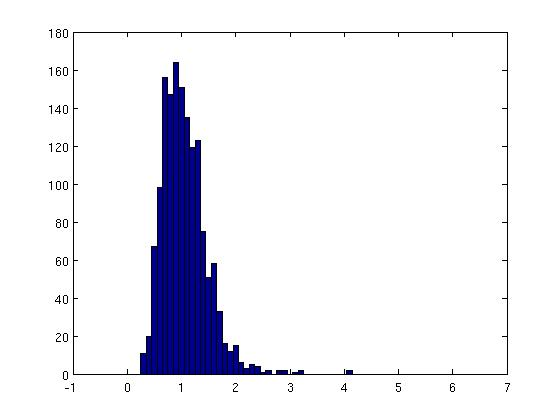
\includegraphics[width=1.5in]{racoon_hist.jpg}}    
   \subfloat[Sea Lions]{\label{fig:sean_lion_hist}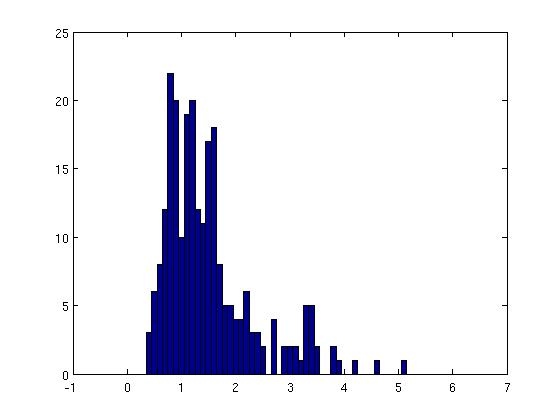
\includegraphics[width=1.5in]{sea_lion_hist.jpg}}    
   \subfloat[Skateboards]{\label{fig:skate_hist}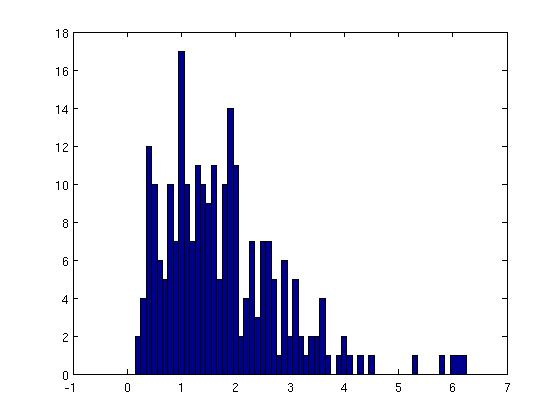
\includegraphics[width=1.5in]{skate_hist.jpg}}    
   \subfloat[Mugs]{\label{fig:mug_hist}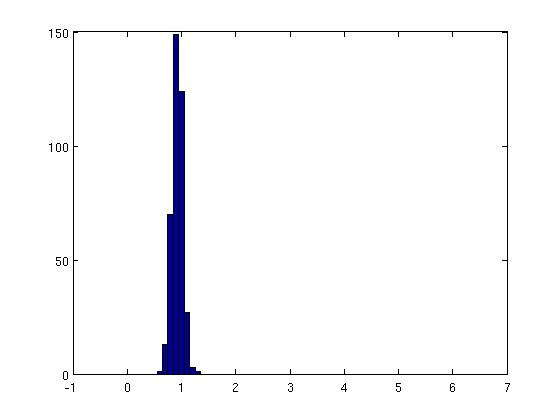
\includegraphics[width=1.5in]{mug_hist.jpg}}    
   \subfloat[Cups]{\label{fig:cup_hist}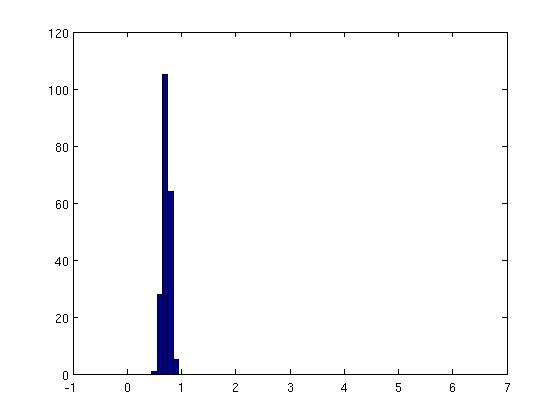
\includegraphics[width=1.5in]{cup_hist.jpg}}    
\end{center}
   \caption{Aspect ratio distributions for different object types across datasets }
\label{fig:histograms}
\end{figure}
%-------------------------------------------------------------------------


\subsection{Simulating sliding window}

As the previous section shows it is a non-trivial task to apply conventional localization
techniques on this dataset. However, without first spending time on developing novel 
localization algorithms we would like to explore the image charecteristics and design
classifiers that learn to recognize that particular class of objects. The approach we use
is to simulate sliding window by extracting the ground truth bounding boxes as positive
images and thousands of non-overlapping snippets from the background as negative images. 
This reduces our problem from a fairly non-trivial object localization problem to a more manageable
object recognition problem where the classifier simply outputs a probability for the existence
of an object in an image. The obvious drawback here is the ratio of the positive versus negative
images since sliding window samples an order of magnitude more negatives. However, if enough
non-overlapping negative snippets are used for every image we can get a close enough approximation
to actually running sliding window in terms of classification performance. To make the sampling of
the negatives as close to real as possible, we assume a Gaussian distribution over the width and height
of the object class, estimate parameters empirically and use those to sample the images.

Figure \ref{fig:sliding} and the equations below shows how an image is broken into positive and negative snippets to simplify the
problem.

\begin{figure}[t]
\begin{center}
   \includegraphics[width=1.8in]{sw.jpg}    
\end{center}
\begin{center}
   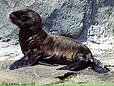
\includegraphics[width=0.5in]{sw_p1.jpg}    
   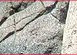
\includegraphics[width=0.5in]{sw_n1.jpg}    
   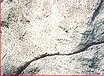
\includegraphics[width=0.5in]{sw_n2.jpg}    
   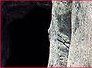
\includegraphics[width=0.5in]{sw_n3.jpg}    
\end{center}
   \caption{Simulating sliding window - an image marked with positive and negative snippets and how they lead to a smaller dataset 
            with the same basic idea}
\label{fig:sliding}
\end{figure}
%-------------------------------------------------------------------------


\[ I = \text{an image from the set of images for class } c \]
\[ G_i^c = \text{set of ground truth bounding boxes for class } c \text{ on image } I \]
\[ P_i^c = \text{set of positive images for simulated sliding window } \]
\[ N_i^c = \text{set of negative images for simulated sliding window } \]
\[ S^c = \text{set of non-overlapping bounding box samples for image } I \]
\[ g^{(j)} , s^{(j)} \epsilon \{ x , y , w , h \} \]
\[ \mu_w = \text{empirical mean of widths for positive snippets } \]
\[ \mu_h = \text{empirical mean of heights for positive snippets } \]
\[ \Sigma_w = \text{empirical variance of widths for positive snippets}  \]
\[ \Sigma_h = \text{empirical variance of heights for positive snippets}  \]
\[\boldsymbol{P_i^c} = \{I({g^{(1)}}),I({g^{(2)}}),\ldots,I({g^{(n)}})\}\]
\[\boldsymbol{N_i^c} = \{I({s^{(1)}}),I({s^{(2)}}),\ldots,I({s^{(n)}})\}\]
\[ {s^{(j)}}(w) \sim Gaussian( \mu_w , \Sigma_w) \]
\[ {s^{(j)}}(h) \sim Gaussian( \mu_h , \Sigma_h) \]
\[ {s^{(j)}}(x) \sim Unif( 0 , I(w) ) \]
\[ {s^{(j)}}(y) \sim Unif( 0 , I(h) ) \]


%-------------------------------------------------------------------------



\subsection{Image Properties}

Before designing classifiers it helps to review some of the basic image properties of all the
positive snippets across a class. In this section we breifly touch upon a few such properties
that are though quite basic but nevertheless useful to share.


\subsubsection{Average and variance}

Figure \ref{fig:prop} simply shows the average and variance images for the different object classes. The objects
were snipped and resized apriori. As excepted based on our initial discussions there is no signal in the
average images and they are extremeley close to being fully grey. The only insight in the variance images
is that there seems to be a lot more variation at the corners that in the middle. This can be taken into
account when developing sampling techniques for image patches. Depending on the application, discriminiative
patches should be extracted more from the sides via an exponential distribution as opposed to generalizable
patches should be extracted more from the middle via a gaussian distribution.

\begin{figure}[t]
\begin{center}
    \subfloat[Sea Lions]{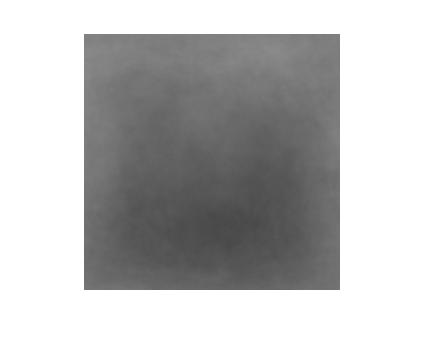
\includegraphics[width=1.8in]{sl_m.jpg}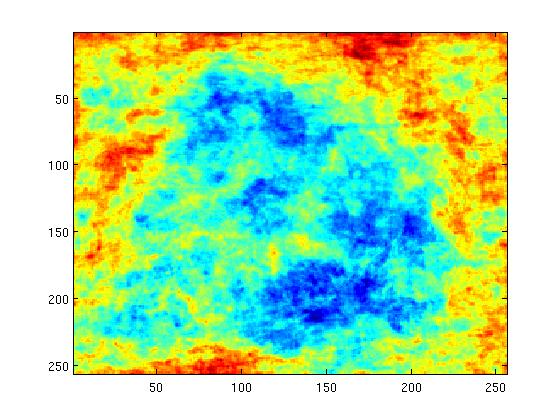
\includegraphics[width=1.8in]{sl_var.jpg}}    
\end{center}
\begin{center}
    \subfloat[Skateboards]{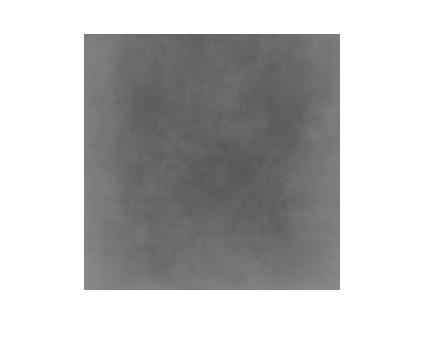
\includegraphics[width=1.8in]{sk_m.jpg}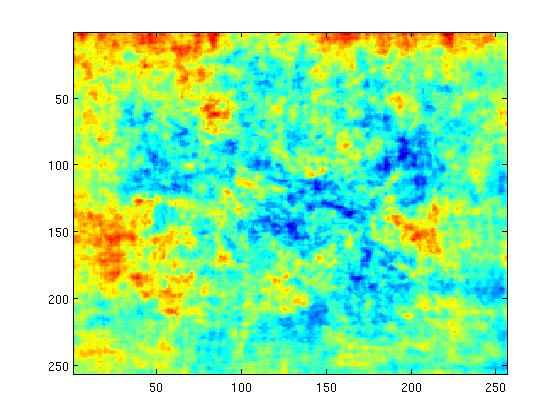
\includegraphics[width=1.8in]{sk_var.jpg}}
\end{center}
\begin{center}
   \subfloat[Racoons]{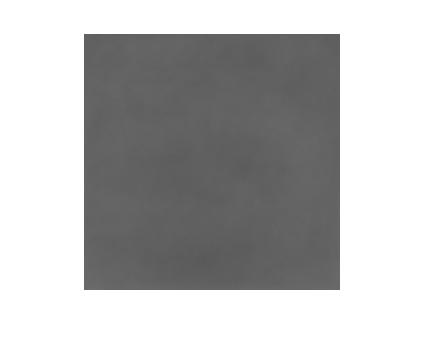
\includegraphics[width=1.8in]{r_m.jpg}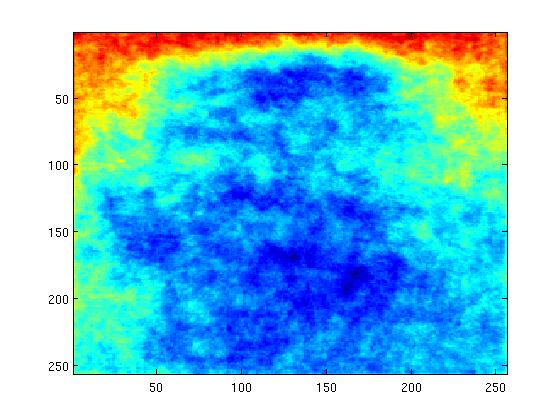
\includegraphics[width=1.8in]{r_var.jpg}}
\end{center}
   \caption{Average images on the left and variance on the right.}
\label{fig:prop}
\end{figure}

\begin{figure}[t]
\begin{center}
    \subfloat[Sea Lions]{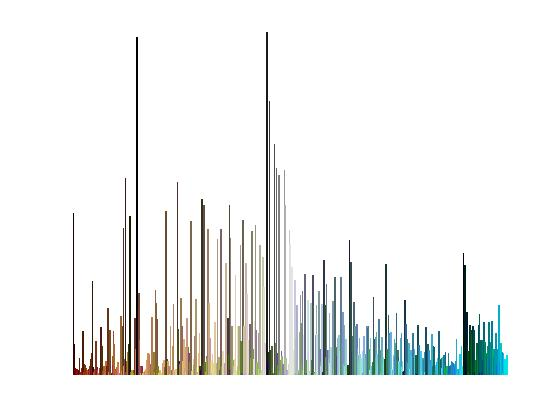
\includegraphics[width=1.8in]{colorh_sl.jpg}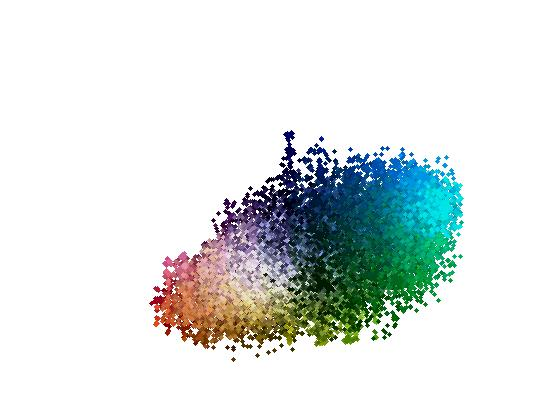
\includegraphics[width=1.8in]{colors_sl.jpg}}    
\end{center}
\begin{center}
    \subfloat[Skateboards]{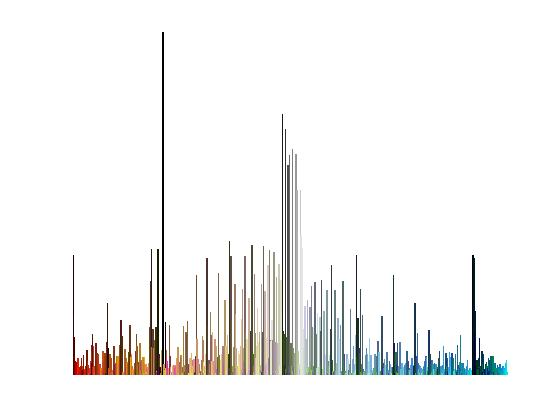
\includegraphics[width=1.8in]{colorh_sk.jpg}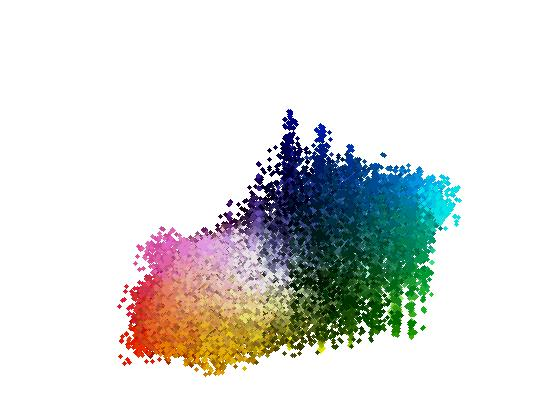
\includegraphics[width=1.8in]{colors_sk.jpg}}
\end{center}
\begin{center}
   \subfloat[Racoons]{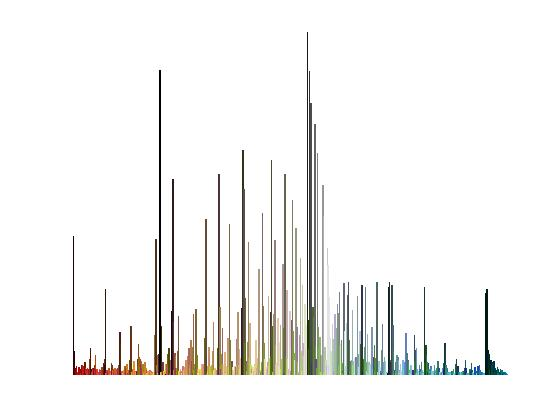
\includegraphics[width=1.8in]{colorh_r.jpg}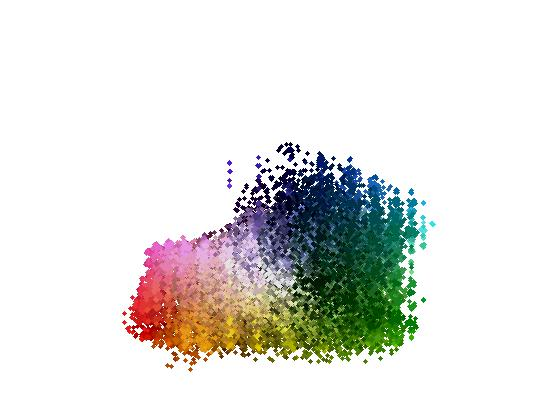
\includegraphics[width=1.8in]{colors_r.jpg}}
\end{center}
   \caption{Color histograms and scatter plots for the different object classes \cite{thirdparty1}.}
\label{fig:color}
\end{figure}

%-------------------------------------------------------------------------

\subsubsection{Color properties}

Eyeballing most datasets can give the false sense that color can be an important feature for recognition
and localization. Historically researchers have avoided the use of color based features for these tasks due to computational
and philosophical reasons. The computational tradeoff is obvious, and the philosophical reason being that humans
can perform these tasks very well without any color information. Figure \ref{fig:color} is a color historgam and a scatter plot of
all the positive snippets of different classes. It shows minor variations for the different classes but no strong
color patterns emerge, atleast globally. There were some interesting insights for designing color features 
when comparing such plots between the positive and negative snippets but for sake of brevity they have been omitted.

%-------------------------------------------------------------------------

\subsection{Classifier design}

Using the simulated sliding window framework described above we present two
different classification strategies based on different features. The experiment
section covers the results and comparisons in details.
%-------------------------------------------------------------------------


\subsubsection{Bag of features}

The is the standard application of the bag of words model applied to image features \cite{bag1,bag2}.
We begin by constructing the codebook. Each positive snippet is densely sampled and a image descriptor
is created at each sampled location. This image descriptor is a 250 dimensional vector which is a combination of the RIFT \cite{feature2}, 
spin images \cite{feature3} and gabor style filter bank \cite{feature4} descriptors. Figure \ref{fig:filter} shows a subset of the filter
banks being used in the image descriptor.
K-Means clustering is used to group similar descriptors in this 250 dimensional space and a codebook is created
by taking each of the K (usually 100-200) cluster centroids descriptors. Equation \ref{eq:fv_bw} shows how the
design matrix is created by the above defined codebook. 

\[\boldsymbol{X} = \{{x^{(1)}}^T,{x^{(2)}}^T,\ldots,{x^{(m)}}^T\} \text{ : design matrix } \]
\[\boldsymbol{D^c} = \{{d^{(1)}}^T,{d^{(2)}}^T,\ldots,{d^{(|D^c|)}}^T\} \text{ : dictionary } \]
\[\boldsymbol{F_i} = \{{f^{(1)}}^T,{f^{(2)}}^T,\ldots,{f^{(|F_i|)}}^T\} \text{ : image descriptors } \]
\[ x(j)^T , d(j)^T , f(j)^T  \epsilon \mathbb{R}^n \]
\begin{equation} 
    {x_j^{(i)}} = {\arg \min}_{f \epsilon F} {||f - {d}^{(j)}||_2}^2 
    \label{eq:fv_bw}
\end{equation}

For each class of objects we use a binary gentle boost classifier over two-split decision stumps and the codebook is trimmed
to remove descriptors not selected by boosting. 
Following this, using cross-validation each unknown image in the test set (under simulated sliding window) is converted to a feature vector and is evalued by the boosted classifier. Results and details are elaborated in the experiment section.
%-------------------------------------------------------------------------

\begin{figure}[t]
\begin{center}
    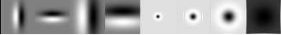
\includegraphics[width=2.0in]{filter.jpg}
\end{center}
\caption{Subset of the filter banks used in the bag of features descriptor.}
\label{fig:filter}
\end{figure}

\subsubsection{Unsupervised codebook generation}

A different approach towards codebook generation is to try and learn one in an 
unsupervised way (i.e. the image descriptors are not manually selected) 
from labelled training data \cite{codebook1}.
The codebook is generated by first densely sampling (well over 100 samples per image) the positive images (under simulated sliding window) and extracting square size patches of sizes varying from 4x4 to 32x32. Similar to the Bag of Features section these patches are linearized and K-Means clustering is applied to find patterns in this data. The codebook then becomes the K (usually 100-150) cluster centroids that are converted back into their original patch form.
Figure \ref{fig:unsupcodebook} shows a set of sample codebook entries. It is interesting to see their similarity with 
Gabor style filter bank features. Although not shown experimentally due to the lack of a concrete metric,
the codebook patches don't generalize well unless a threshold number of images are used and or a threshold
number of patches are extracted for the K-Means clustering.

\begin{figure}[t]
\begin{center}
    \subfloat[Sea Lions]{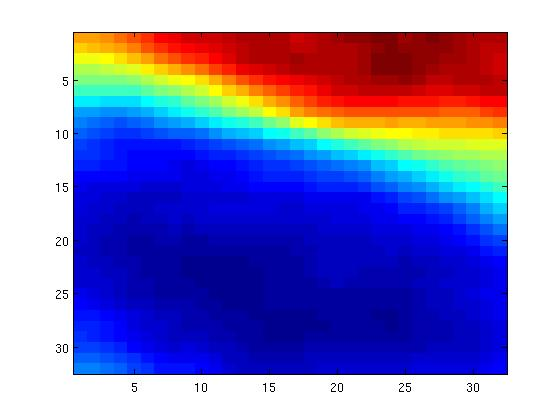
\includegraphics[width=0.6in]{sl_d1.jpg}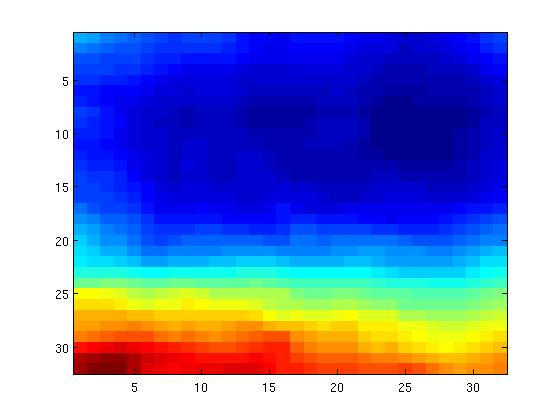
\includegraphics[width=0.6in]{sl_d2.jpg}
                         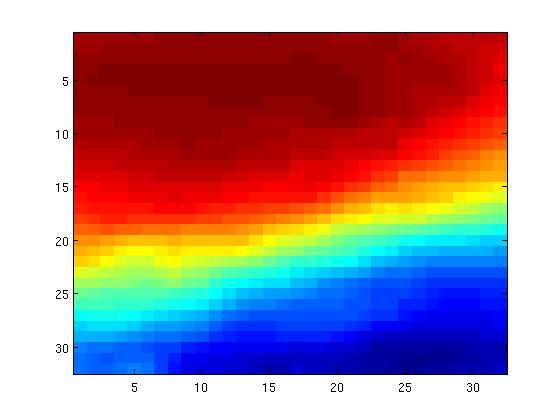
\includegraphics[width=0.6in]{sl_d3.jpg}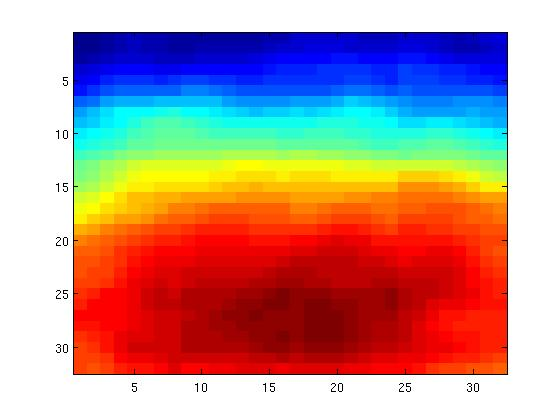
\includegraphics[width=0.6in]{sl_d4.jpg}
                         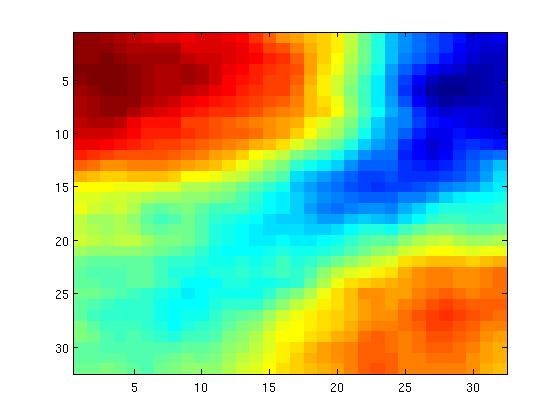
\includegraphics[width=0.6in]{sl_d5.jpg}
                        }
    \subfloat[Skateboards]{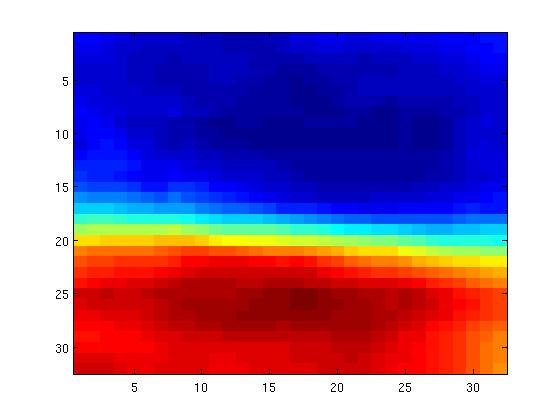
\includegraphics[width=0.6in]{sk_d1.jpg}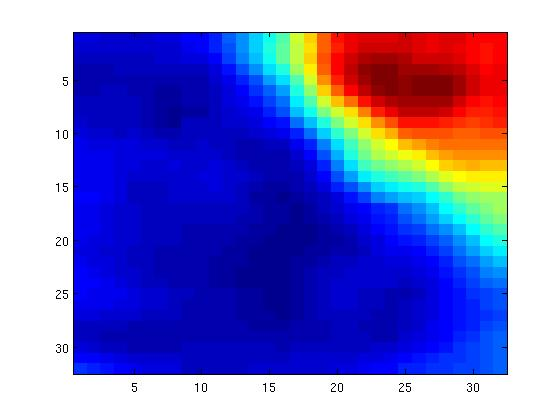
\includegraphics[width=0.6in]{sk_d2.jpg}
                         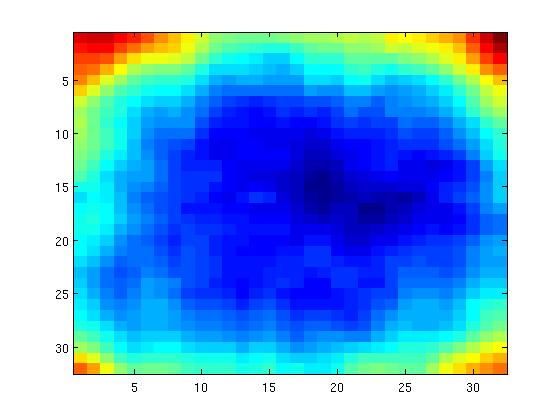
\includegraphics[width=0.6in]{sk_d3.jpg}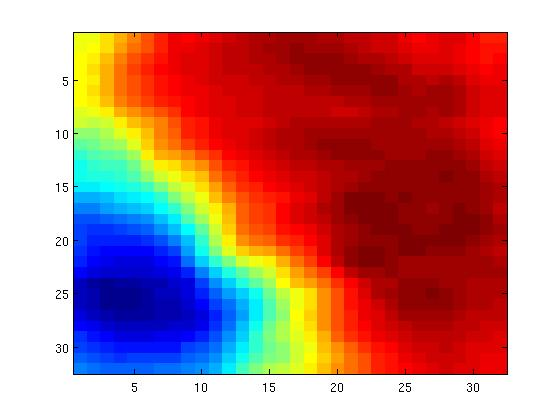
\includegraphics[width=0.6in]{sk_d4.jpg}
                         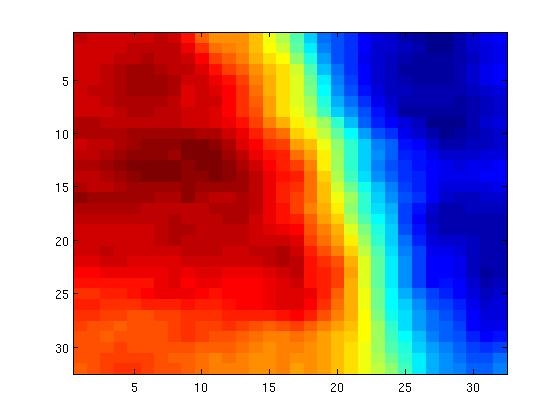
\includegraphics[width=0.6in]{sk_d5.jpg}
                        }
    \subfloat[Racoons]{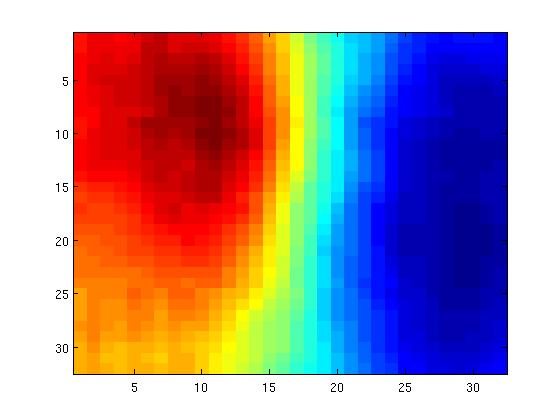
\includegraphics[width=0.6in]{r_d1.jpg}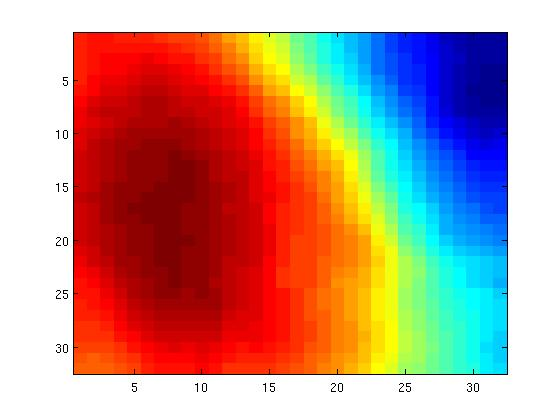
\includegraphics[width=0.6in]{r_d2.jpg}
                         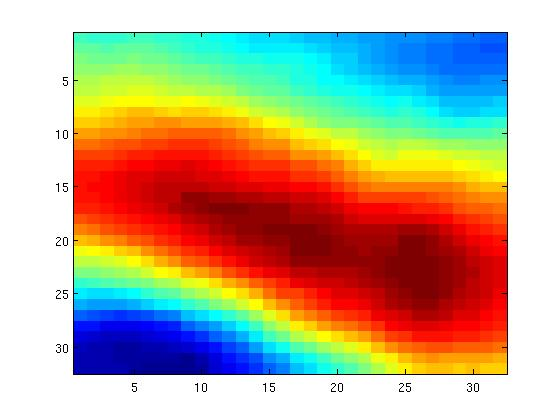
\includegraphics[width=0.6in]{r_d3.jpg}\includegraphics[width=0.6in]{r_d4.jpg}
                         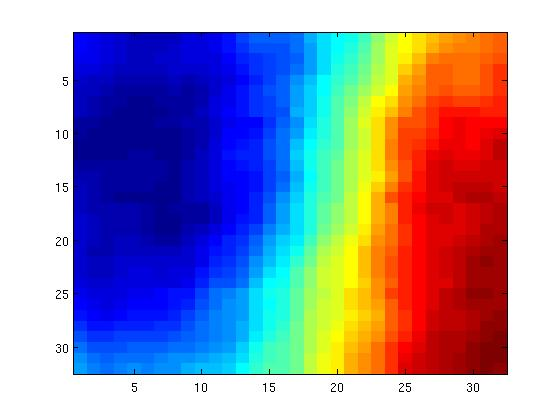
\includegraphics[width=0.6in]{r_d5.jpg}
                        }
\end{center}
   \caption{Randomly selected codebook entries.}
\label{fig:unsupcodebook}
\end{figure}

%-------------------------------------------------------------------------

Equation \ref{eq:fv_cb} shows how the design matrix is created using the max reponses of each of these codebook patches. 
For each class of objects an SVM classifier is trained using the design matrix.
Following this, cross-validation is used and each unknown image in the test set is converted to a feature vector and evaluated by the SVM classfier. 

\[\boldsymbol{X} = \{{x^{(1)}}^T,{x^{(2)}}^T,\ldots,{x^{(m)}}^T\} \text{ : design matrix } \]
\[\boldsymbol{D^c} = \{{d^{(1)}},{d^{(2)}},\ldots,{d^{(|D^c|)}}\} \text{ : dictionary } \]
\[ x(j)^T  \epsilon \mathbb{R}^n \]
\[ d(j)  \epsilon \mathbb{R}^{32 \times 32} \]
\begin{equation} 
    {x_j^{(i)}} = {\max}( I \bigotimes d^{(j)}) 
    \label{eq:fv_cb}
\end{equation}

%-------------------------------------------------------------------------

\subsection{A Boosting Inspired Approach to Localization}

After having highlighted the apparent drawbacks of applying conventional object
localization techniques on the ImageNet dataset we now present an approach to
localization inspired by the boosting algorithm.  

It is used along with the unsupervised codebook approach illustrated in the previous section.
Each individual codebook entry is hypothesised to be a "weak vote" of where the
object instances within the image are located much like each codebook entry is a 
weak classifier in the boosting framework. Instead of simply taking the best response
of each codebook entry as a vote we take the top few responses on the image (the image here
is the entire image and not a positive or negative snippet) and weigh them by the value of
the response. 

\[\boldsymbol{X} = \{{x^{(1)}}^T,{x^{(2)}}^T,\ldots,{x^{(m)}}^T\} \text{ : locations in image space } \]
\[\boldsymbol{D^c} = \{{d^{(1)}},{d^{(2)}},\ldots,{d^{(|D^c|)}}\} \text{ : dictionary } \]
\[\boldsymbol{W} = \{W_1,W_2,\ldots,W_n \} \text{ : set of weight matrices } \]
\[ x(j)^T  \epsilon \mathbb{R}^2 \]
\[ d(j)  \epsilon \mathbb{R}^{32 \times 32} \]
\[ W_j \epsilon \mathbb{R}^{I(w) \times I(h)} \]
\[ W_j  = I \bigotimes d^{(j)} \] 

\textbf{Modified K-Means}\newline

For each location (i) :

\[ c^{(i)} = \arg \min {|| {W_j}^{(i)} * x(i) - \mu_j ||_2}^2 \]

For each cluster centroid (j) :

\[ \mu_j =  \frac{\sum_{i=1}^{m}1\{c^{(i)} = j\}{W_j}^{(i)} * x^{(i)}}{\sum_{i=1}^{m}1\{c^{(i)} = j\}} \]

The main intuition behind the localizing process comes from the boosting framework which
suggests that the sum of all the weak classifiers in the system becomes a strong classifier.
Similar to this idea, we make a hypothesis that each patch response is a weak vote of the
location of the object and a combination of all these weak votes should become a strong vote.
A variation of the K-Means clustering process is used to identify the clusters amongst these
votes. We then use the statistics of these clusters (the mean and variance)
to try and estimate an ellipse signifying the position of the object which is then trivially converted
to a rectangle for comparison with the ground truth.\newline 

\textbf{Forming Ellipses from Cluster Centroids} \newline

For each cluster centroid (j) :

\[ [width_j , height_j] =  \frac{\sum_{i=1}^{m}1\{c^{(i)}=j\} (\mu_j - {W_j}^{(i)} * x(i))^2 }{\sum_{i=1}^{m}1\{c^{(i)}=j\}} \]
\[ [x_j , y_j] = \mu_j \]

Although this approach doesn't provide state of the art results it is interesting to see the
overall insights about the kind of approaches and features that work and those that don't work.


%-------------------------------------------------------------------------

\section{Experiment}

Figure \ref{fig:dataset} gave a small peek at the complexity involved in the chosen ImageNet
categories. There are three object classes for sealions, skateboards and racoons, with 165, 229 and
1182 images respectively. All images were labelled to draw bounding boxes around the object instances
within these images and these were treated as the ground truth. For the simulated sliding window
approach these snipped ground truth boxes became the positive images and around 100 negative snippets
per image became the negative images. The results for the bag of features boosted classifier and
the unsupervised codebook SVM classifier were all based off the simulated sliding window dataset.

Figure \ref{fig:fv_bw} shows the a few chosen features from a feature vector plot for the bag of features model. 
Using the design matrix generated from equation \ref{eq:fv} we create each coordinate in this plot based on
the equations below:

\begin{figure}[t]
\begin{center}
    \subfloat[Sea Lions]{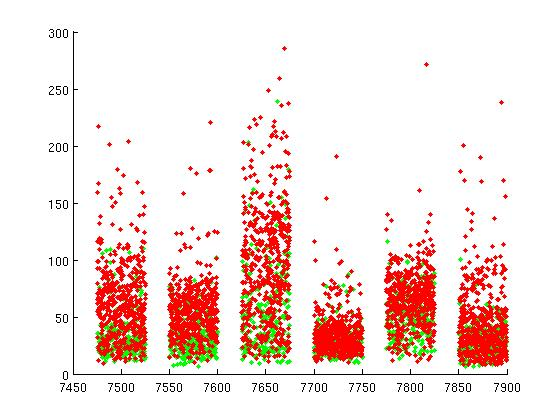
\includegraphics[width=1.8in]{sl_fv.jpg}
                        }
    \subfloat[Skateboards]{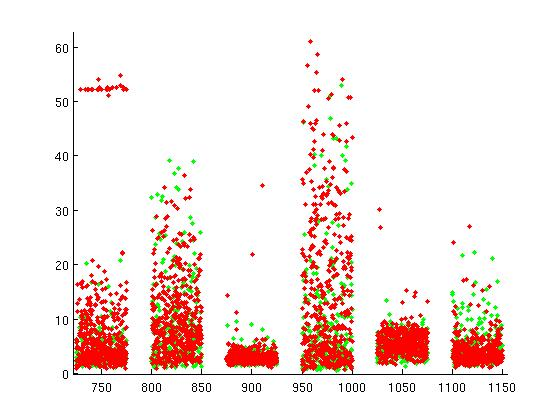
\includegraphics[width=1.8in]{sk_fv.jpg}
                        }
    \subfloat[Racoons]{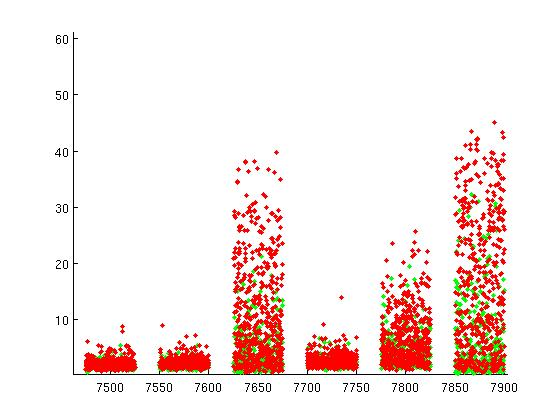
\includegraphics[width=1.8in]{r_fv.jpg}
                        }
\end{center}
   \caption{Feature vector plots for 6 randomly selected features from the bag of features model.}
\label{fig:fv_bw}
\end{figure}

Notice how mixed the feature vector values for the positive and negative images are in most of the features
shown. This implies that a learning algorithm will have a hard time find a seperating boundary for these features.
Very few features actually offer some separation.

Figure \ref{fig:fv_cb} shows a similar feature vector plot for the design matrix also generated via
equation \ref{eq:fv} in the unsupervised codebook model. Its interesting to see that a lot of 
the features shown offer a decent separation and hence this model should imply a much
better performance. This intuition is confirmed empirically in the results ahead.

\begin{figure}[t]
\begin{center}
    \subfloat[Sea Lions]{\includegraphics[width=1.8in]{sl_fv_p.jpg}
                        }
    \subfloat[Skateboards]{\includegraphics[width=1.8in]{sk_fv_p.jpg}
                        }
    \subfloat[Racoons]{\includegraphics[width=1.8in]{r_fv_p.jpg}
                        }
\end{center}
   \caption{Feature vector plots for 6 randomly selected features from the unsupervised codebook model.}
\label{fig:fv_cb}
\end{figure}

\[\boldsymbol{X} = \text{ design matrix from equation \ref{eq:fv_bw} or \ref{eq:fv_cb} } \]

For each entry \begin{math} {x_j}^{(i)} \end{math} in the design matrix \begin{math} \boldsymbol{X} \end{math}

\[ s^{(i)} \sim Unif(-10,10) \]
\begin{equation} 
    [row^{(i)} ,  col^{(i)}] = [ {x_j}^{(i)}  , s + j] 
    \label{eq:fv}
\end{equation}

Table \ref{tab:acc_bw} shows the results of the 20-fold cross validation on the simulated sliding window
dataset using the two classifiers discussed above.
 
 \begin{table}
   \begin{center}
    \begin{tabular}{ | l | l | l | }
    \hline
    \textbf{Object} & \textbf{Bag of Words} & \textbf{Unsupervised Codebook}  \\ \hline
    Sea Lions & 0.450 & 0.9350 \\ \hline
    Skateboards & 0.162 & 0.6920 \\ \hline
    Racoons & 0.944 & 0.9228 \\ \hline
    \end{tabular}
    \caption{Accuracy of the classifiers on the simulated sliding approach set.}
    \label{tab:desc}
    \end{center}
  \end{table}
 
Figure \ref{fig:boost_rounds} is the change in accuracy (using cross-validation) for the different classes 
as the number of boosted round increase.

\begin{figure}[t]
    \includegraphics[width=3.5in]{boosting_rounds.jpg}
   \caption{Accuracy versus number of boosting rounds. RGB is sea lion, skateboards and racoons respectively.}
   \label{fig:boost_rounds}
\end{figure}

It is interesting to note the effective of the different image descrptors individually as shown in
Table \ref{tab:desc}. They seem to share very complementary to each other and hence the combined accuracy
is much higher that their individual accuracy.
 
 \begin{table}
   \begin{center}
    \begin{tabular}{ | l | l | l | l | l |}
    \hline
    \textbf{Object} & \textbf{RIFT} & \textbf{SPIN} & \textbf{Filters} & \textbf{All}  \\ \hline
    Sea Lions & 0.400 & 0.406 & 0.414 &  0.450 \\ \hline
    Skateboards & 0.152 & 0.169 & 0.1742 & 0.163 \\ \hline
    Racoons & 0.491 & 0.469 & 0.486 & 0.944 \\ \hline
    \end{tabular}
    \caption{Accuracy of the classifiers using variants of the bag of features model.}
    \label{tab:acc_bw}
    \end{center}
  \end{table}


It is also interesting to note the impact of the size of the bag of features codebook i.e. number of
cluster centroids on the overall
performace of the different classifiers as noted in Figure \ref{fig:code_size}

\begin{figure}[t]
    \includegraphics[width=3.5in]{codebook_size.jpg}
   \caption{Accuracy versus size of codebook for the bag of features model. RGB is sea lion, skateboards and racoons respectively.}
   \label{fig:code_size}
\end{figure}

For testing the boosting inspired localization approach we used the same unsupervised codebook as used
for the above experiments and chose a completely seperate test set of complete images (not snipped ones)
that contain one or more instanes of the object class. The set was of 100 images for each object
class and the accuracy reported in Table \ref{tab:local}. A detection outputted by our algorithm is considered
as correct if \begin{math} (D \cap G) / max( D ,G ) \end{math} is greater than \begin{math}0.6\end{math}
where \begin{math}D\end{math} is a detection and \begin{math}G\end{math} is a ground truth bounding box.
 
 \begin{table}
   \begin{center}
    \begin{tabular}{ | l | l | l | }
    \hline
    \textbf{Object} & \textbf{Accuracy}  \\ \hline
    Sea Lions & 0.333 \\ \hline
    Skateboards & 0.111  \\ \hline
    Racoons & 0.504  \\ \hline
    \end{tabular}
    \caption{Localization accuracy for the proposed boosting inspired approach.}
    \label{tab:local}
    \end{center}
  \end{table}

Figure \ref{fig:final} shows some results (good and bad) of the boosting inspired localization algorithm for the
different classes. Skateboards are by far the hardest class to accurately localize, this could be because
of the lack of strong, large generalizable features. In most error cases the actual skateboards within the images are
simply too small or thin
for the image descriptors of both types to actually find a singal. In the case of sea lions their appearance
, pose and view-point variation is enormously large and hence hard to work with. Racoons perhaps worked the best
because of a relatively stable appearance which allows the descriptors to find a consistent signal.

\begin{figure*}
\begin{center}
    \includegraphics[width=2in]{loc_sl_1.jpg}
    \includegraphics[width=2in]{loc_sl_2.jpg}
    \includegraphics[width=2in]{loc_sl_3.jpg}
    \includegraphics[width=2in]{loc_sl_4.jpg}
    \includegraphics[width=2in]{loc_sl_5.jpg}
    \includegraphics[width=2in]{loc_sl_6.jpg}
\end{center}
\begin{center}
    \includegraphics[width=2in]{loc_r_1.jpg}
    \includegraphics[width=2in]{loc_r_2.jpg}
    \includegraphics[width=2in]{loc_r_3.jpg}
    \includegraphics[width=2in]{loc_r_7.jpg}
    \includegraphics[width=2in]{loc_r_8.jpg}
    \includegraphics[width=2in]{loc_r_6.jpg}
\end{center}
\begin{center}
    \includegraphics[width=2in]{loc_sk_1.jpg}
    \includegraphics[width=2in]{loc_sk_2.jpg}
    \includegraphics[width=2in]{loc_sk_3.jpg}
    \includegraphics[width=2in]{loc_sk_4.jpg}
    \includegraphics[width=2in]{loc_sk_5.jpg}
    \includegraphics[width=2in]{loc_sk_6.jpg}
\end{center}
   \caption{Localization results}
\label{fig:final}
\end{figure*}

%------------------------------------------------------------------------



%-------------------------------------------------------------------------

\section{Conclusion}

We once again reiterate the general theme of this paper that the ImageNet dataset
due to its sheer number of images per category is a very good approximation to
the true real world variability in object attributes such as apperance, shape,
pose, view point, size etc. The paper highlights some of these complexities
and provides insights which may help in deciding an approach
to this challenging problem. We presented a boosting inspired localization approach
which is although not state of the art but it gives insight into the kind of localization
methods that will work as opposed to the conventional ones. An unsupervised
codebook provides the best performance out of all the feature descriptors used. It may be
very interesting to see how a heirarchical codebook improves the efficiency - almost like
a deep belief network where the "codebook" of a higher layer could implicitly model the
parts of highly deformable objects like animals for it is quite clear that lower
level image features will not be able to come close to truly solving this problem. Heirarchical
codebooks also will not individually scale for each object type so it will be fruitful to think of approaches
that share codebooks similar to the work in \cite{multiview4} so that we can think of efficient
scaling as well. Lastly, studies on the impact of sharing codebooks and object parts based on the
ontologies in ImageNet is an intruiging work for the future.

%-------------------------------------------------------------------------


{\small
\bibliographystyle{ieee}
\bibliography{egbib}
}

\end{document}
